\section{Methodology}	
When dealing with natural language, our main purpose is to make computer understand the rules and formation of
natural language. How a sentence built and how each parts of the sentences are connected with each other. To make computer understand about the human level natural language, we have to design a Natural Language Processing(NLP) Pipeline.\\ 
	
After understanding the given text, we have to make choices that how could we do the task that is instructed in the text. So we need a learning environment by which we can teach our agent(robot) to execute the task. Our task
here is to generate the necessary actions to accomplish the task.\\
	
As in this work we're navigating a robot via natural language instruction, so we also need an environment
where we can view and observe the environment around the robot and give instructions in accordance.\\
	
So in this work our methodology is centered on three key point: A NLP Pipeline, A Learning Algorithm and A Navigation Environment. \\

\subsection{Work Already Done}

\subsubsection{NLP Pipeline Designing}

The first stage of our work is the designing of a NLP pipeline. The steps associated with designing a NLP pipeline are as follows: \\

\begin{enumerate}
    \item Sentence Segmentation
    \item Word Tokenization
    \item Predicting Parts of Speech for Each Token
    \item Text Lemmatization
    \item Identifying Stop Words
    \item Dependency Parsing
    \begin{enumerate}
        \item Finding Noun Phases
    \end{enumerate}
    \item Named Entity Recognition (NER)
\end{enumerate}
\vline

Now we should focus on a brief discussion of these steps. We consider the sentence: "Go near the red triangle. Wait for three seconds. Then go to green rectangle."\\

\paragraph{Sentence Segmentation}
The first step in the pipeline is to break the text apart into separate sentences. Thus gives us this:
\begin{enumerate}
    \item "Go near the red triangle."
    \item "Wait for three seconds."
    \item "Then go to green rectangle."
\end{enumerate}

\paragraph{Word Tokenization}
Now that we’ve split our document into sentences, we can process them one at a time. The next step in our pipeline is to break this sentence into separate words or tokens. This is called tokenization. This is the result: \\

\begin{tabular}{|p{10cm}}
    "Go", "near", "the", "red", "triangle", "." 
\end{tabular}\\
\vline


Tokenization is easy to do in English. We’ll just split apart words whenever there’s a space between them. And we’ll also treat punctuation marks as separate tokens since punctuation also has meaning.

\paragraph{Predicting Parts of Speech for Each Token}
Next, we'll look at each token and try to guess its part of speech-whether it is a noun, a verb, an adjective and so on. Knowing the role of each word in the sentence will help us start to figure out what the sentence is talking about.\\

We can do this by feeding each word (and some extra words around it for context) into a pre-trained part-of-speech classification model. The part-of-speech model was originally trained by feeding it millions of English sentences with each word’s part of speech already tagged and having it learn to replicate that behavior.\\

After processing the whole sentence, we'll have result like this:
\begin{table}[h]
    \centering
    \begin{tabular}{ccccc}
        Go   & near      & the        & red  & triangle \\
        Verb & Adjective & Determiner & Noun & Noun    
    \end{tabular}
\end{table}

\paragraph{Text Lemmatization}
In English (and most languages), words appear in different forms. When working with text in a computer, it is helpful to know the base form of each word so that we know both sentences are talking about the same concept. In NLP, we call finding this process lemmatization-figuring out the most basic form or lemma of each word in the sentence. The same thing applies to verbs. We can also lemmatize verbs by finding their root, unconjugated form. Lemmatization is typically done by having a look-up table of the lemma forms of words based on their part of speech and possibly having some custom rules to handle words that we’ve never seen before.
\paragraph{Identifying Stop Words}
Next, we want to consider the importance of a each word in the sentence. English has a lot of filler words that appear very frequently like “and”, “the”, and “a”. When doing statistics on text, these words introduce a lot of noise since they appear way more frequently than other words. Some NLP pipelines will flag them as stop words —that is, words that you might want to filter out before doing any statistical analysis.

\paragraph{Dependency Parsing}
The next step is to figure out how all the words in our sentence relate to each other. This is called dependency parsing.\\

The goal is to build a tree that assigns a single parent word to each word in the sentence. The root of the tree will be the main verb in the sentence.\\

It’s also important to remember that many English sentences are ambiguous and just really hard to parse. In those cases, the model will make a guess based on what parsed version of the sentence seems most likely but it’s not perfect and sometimes the model will be embarrassingly wrong. But over time our NLP models will continue to get better at parsing text in a sensible way.
\subparagraph{Finding Noun Phrases}
So far, we’ve treated every word in our sentence as a separate entity. But sometimes it makes more sense to group together the words that represent a single idea or thing. We can use the information from the dependency parse tree to automatically group together words that are all talking about the same thing.

\paragraph{Named Entity Recognition (NER)}
The goal of Named Entity Recognition, or NER, is to detect and label the nouns with the real-world concepts that they represent. But NER systems aren’t just doing a simple dictionary lookup. Instead, they are using the context of how a word appears in the sentence and a statistical model to guess which type of noun a word represents.\\

Here are just some of the kinds of objects that a typical NER system can tag: People’s names, Company names, Geographic locations (Both physical and political), Product names, Dates and times, Amounts of money, Names of events.\\
In our environment we'll tag certain locations of the environment.\\


\subsubsection{Action Generation}
For navigating in the environment, our agent has to develop or generate actions for the given instructions. Currently we use the basic reinforcement learning algorithm: Value Iteration to generate actions for the agent.\\

Value Iteration algorithm works in a grid environment where we've one or more rewards and one or more punishments in some grids. According to that reward or punishment we generate value for each action for each grid. The formula associated with value iteration algorithm is as follows:\\

$V^*(s) = \max \sum T(s, a, s')[R(s, a, s')  + \gamma V^*(s')]$\\

An example of a $3 X 3$ grid with optimal policy and optimal values after applying value iteration is given in the following image.\\


\begin{figure}[ht]
    \centering
    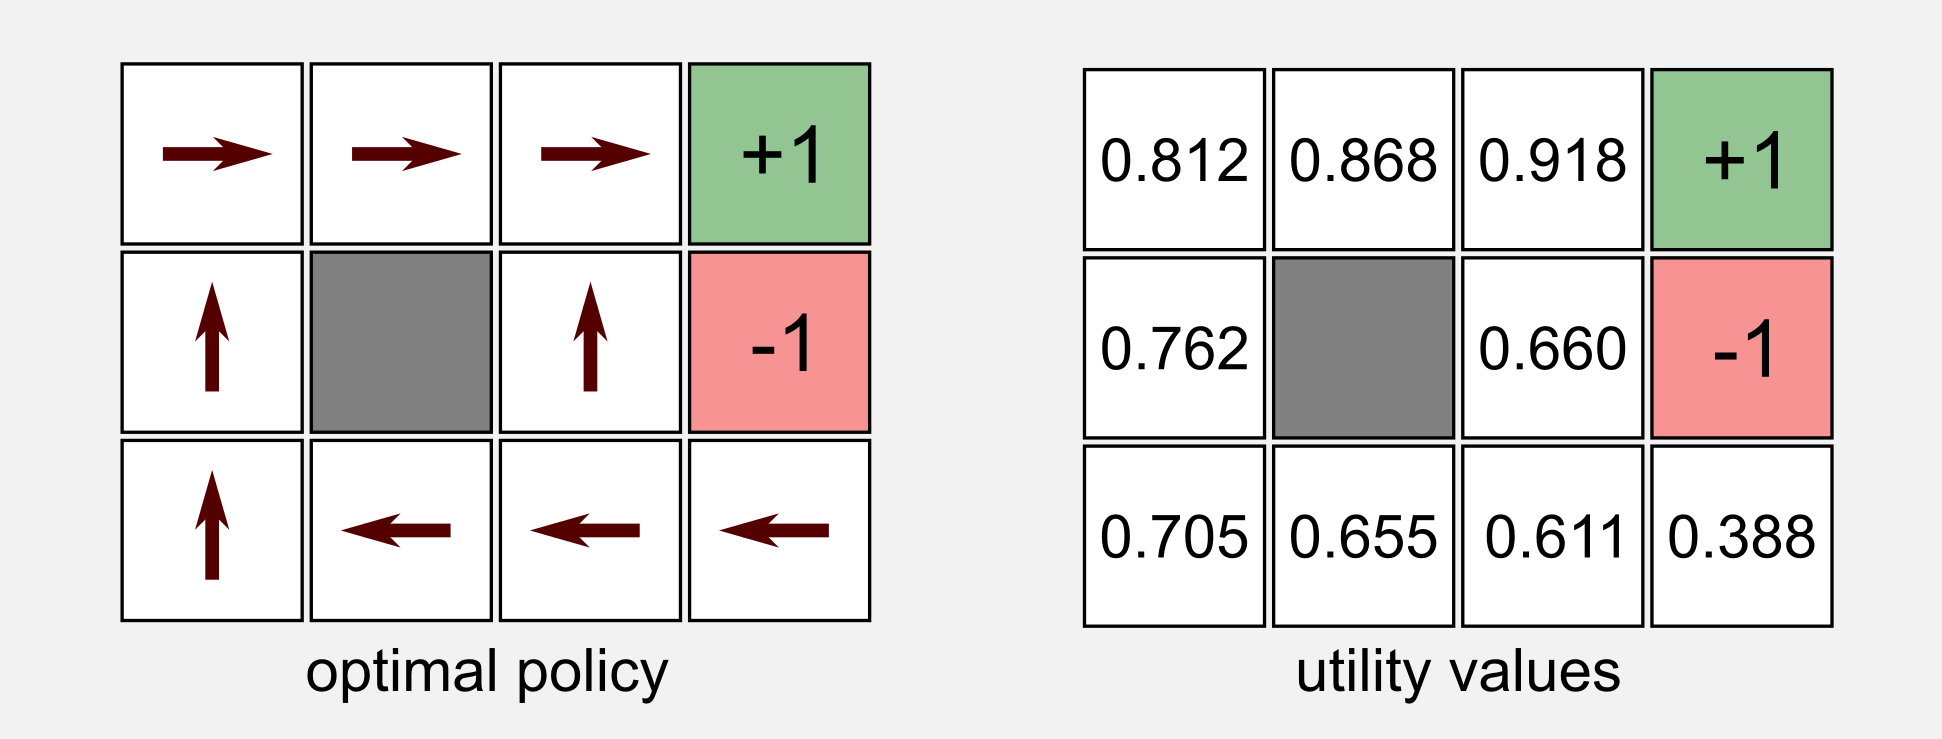
\includegraphics[scale=0.5]{value_iteration}
    \caption{Value Iteration Example}
\end{figure}
\vline

For using the Value Iteration algorithm we split our environment in $25 X 35$ grids. We set reward in grids which is our destinations. We decrease reward value according to the hierarchy or the destination. Similarly we set negative reward in the grid that we should have to avoid.\\

After iterating the algorithm over the whole grid several time we can get the optimal action for each grid. According to this optimal option, agent(robot) will start moving.\\


\subsubsection{Environment Designing}
For now we've used a simple graphical interface to describe the environment and observe the movement of the agent. We should give navigation instruction according to the given environment.

\begin{figure}[h]
    \centering
    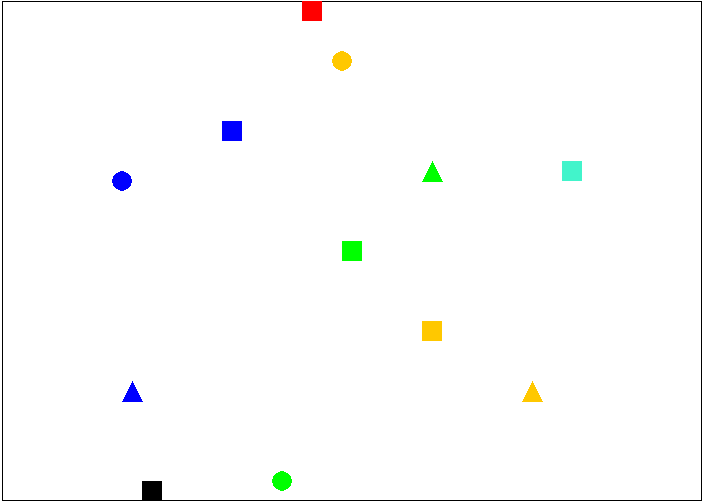
\includegraphics[scale=0.5]{environment}
    \caption{Currently Used Environment}
\end{figure}
\vline

\subsection{Expected Work to be Done}

\subsubsection{NLP Pipeline Designing}
What pipeline we've already designed is moderately enough for language processing tasks. We didn't use the whole pipeline as our used navigation environment is still not much complex. With the increasing complexity of the navigation environment, input instructions will be complex. So for our upgraded version of this project we'll need this whole NLP pipeline.\\

We've designed our NLP pipeline for English language. But as our project aims to navigate robot using Bengali language, we've needed some special consideration for Bengali NLP pipeline. We've to convert the whole pipeline such a way that it could process Bengali language.


\subsubsection{Action Generation}
We aim to develop a Machine Learning model to generate action from a given instruction. This is the core part of our project. For training machine learning model we need data of our environment. As we still didn't design the complex and complete environment we don't have those data right now.\\

After completing the designing of the environment, we use the navigation instruction data to to train our model to generate actions.

\subsubsection{Environment Designing}
We want to design an environment with real life element like tree, building etc. We want to represent the environment via a graphical interface.\\

Alongside the graphical interface we also demonstrate the environment in real life with some dummy element like toy car or toy tree. We want to synchronize the navigation of real life demo in our graphical interface too.\\

After completing the design of the environment and above mentioned two other steps we hope to have our project ready completely. 
